\documentclass[twocolumn]{article}

\title{Evaluation}
\usepackage{graphicx}
\usepackage[margin=0.75in]{geometry}
\usepackage{subcaption}
\usepackage{float}
\usepackage{blindtext}

\graphicspath{ {graphs/} }

\addtolength{\topmargin}{0.25in}
	\addtolength{\textheight}{-0.5in}

\begin{document}

\section[1]{Related Work}
	There are many existing tools that closely relate to Flair in their goals. We provide an overview of the most prevalent of those tools below:
	\subparagraph{Covert}
		Covert is a tool for the compositional analysis of inter-application communication in Android. It allows for the anaylsis of both single applications and bundles of applications. It extracts the source code from each application, extracts communication and security information, and runs formal anaysis on that information to identify any inter-app vulnerabilities.\cite{Covert}.
	\subparagraph{DidFail}
		Didfail is an Android security system built on \textit{FlowDroid} and \textit{Epicc} focused on identifing both inter an intra-compnent vulnerabilities in bundles and individual applications. Didfail first identifies what communications allowed by each individual application. It then analyzes these possible communication to determine any vulnerabilties that may be present in the bundle or application.\cite{Didfail}
	\subparagraph{DIALDroid}
		DIALDroid is an inter-application ICC security analysis system aimed at the analysis of extremely large bundles of applications. It identifies ICC leaks and privelege escalations within large bundles of applications. DIALDroid extracts permisions and possible inter-component communications from the APK files and then analyzes that extracted information. This analysis' percision is varies based on the time the application takes to complete. If the analysis of an application is not complete in a specified time limit, DIALDroid switches to a low precision analysis. If the low precision analysis does not complete within another specified time limit, the analysis is abandoned altogether. After the analysis of all applications in a bundle, the results are stored in a MySQL database to be retrieved when requested.\cite{DIALDroid}.
	\subparagraph{SEALANT}
		SEALANT is an android security system with the goal of both finding and preventing malicious android activity. It is composed of two tools: an analyzer and an interceptor. In this paper we focus only on the analyzer tool as it is closely related to our research. The analyzer works similarly to other ICC analysis tools. First, it extracts ICC paths from APK files. It then identifies vulnerable paths using formal analysis. Lastly, it enters the identified vulnerabilities into a list that will be used by the SEALANT interceptor tool.


\begin{center}
\section[2]{Empirical Evaluation}
\end{center}

\paragraph{•}
	We tested Flair's performance in relation to the following questions:\\
	\textbf{RQ1:} How does Flair compare to other inter-application communication analysis tools in respect to the amount of time it takes to analyze a bundle of applications?\\
	\textbf{RQ2:} How accurately does Flair analyze privilege escalation vulnerabilities within applications when ran against a bundle of benchmark applications?\\
	\textbf{RQ3:} How does Flair's accuracy in analyzing privilege escalations compare to other inter-application communication analysis tools?\\

\subsection{Methods of Testing} \label{methods}
\paragraph{•}
	To test these questions we ran Flair four other inter-application analysis tools: Covert, Didfail, SEALANT, and DIALDroid. We used seven bundles of popular applications presented in table 1, each with fifty applications, to answer RQ1. We then used two bundles of benchmark bundles also presented in table 1 to answer RQ2 and RQ3. 

\begin{table}[h]
\begin{center}
\begin{tabular}{ |c c| }
	\hline
	Bundle & Apks\\
	\hline
	Android Bundle 1 & 50\\
	Android Bundle 2 & 50\\
	Android Bundle 3 & 50\\
	Android Bundle 4 & 50\\
	Android Bundle 5 & 50\\
	Android Bundle 6 & 50\\
	Android Bundle 7 & 50\\
	DroidBench2.0 & 3\textbf{(Not Final)}\\
	ICC-Bench & 9\\
	\hline
\end{tabular}
\end{center}
\caption{Bundles used in analysis.}
\label{table:1}
\end{table}


\paragraph{•}
	Each test we ran to examine RQ1 was incremental in nature. A shell script was utilized to copy each application from a given bundle into a specific input directory. The shell script would then call a tool to be run against that input directory. Each application from a given bundle was copied one by one into the input directory, and the tool was run after each application was copied. This resulted in each test for a given bundle and tool to have 50 total runs. The order in which the bundles were copied into the input directories of each tool remained constant allowing the times outputted to be compared directly. 
\paragraph{•}
	To investigate RQ1 we ran the test described above and recorded the time it took for the tools to analyze the bundles. At every step in the iterative process the time was recorded before the tool was run against the input directory and after the analysis was completed. These times were then written to a CSV file. Each test outputted its times to a single CSV file and the times from all tests were then combined into a master spreadsheet. These times were translated into graphs and are presented later in this paper.\\
	In addition to analyzing the time it took each tool to analyze the bundles. We also noticed that DIALDroid would fail to analyze some applications. Each time it would fail to analyze an application it would output an error log file. After each test we would calculate the failure rate with the following calculation:\\
	\begin{center}
		\(\frac{failed}{num}=FR\)
	\end{center}
	Where \textit{failed} is the number of error logs given by the tool, \textit{num} is the total number of applications run in the test, 1250, and \textit{FR} is the failure rate  in that test. These failure rates were recorded and averaged. We did not notice any of the other tools failing to analyze applications during our tests.
\paragraph{•}
	
	\textbf{Here will go text explaining RQ3 procedure.}
\paragraph{•}
	\textbf{Here will go text explaining Question 4 procedure.}

\subsection{Variables}
\paragraph{•}
	\textbf{Independent:} Our independent variables present in our test are as follows: (1) Tool used to analyze. (2) Specific bundle which the tool analyzed.\\
	\textbf{Dependent:} The dependent variables in our study are as follows: (1) Time it takes for tool to analyze a bundle. (2) Number of applications that a tool fails to analyze. (3) The accuracy of the analysis.
	
\subsection{Testing Environment}
	All testing for Question 1 and RQ2 was done on virtual machines running within Oracle VirtualBox. Each of these machines was running Ubuntu 16.04 and had 8 processing threads clocked at 2.28 Ghz. The memory varied due to the fact that each tool had differing memory requirements. For Covert, Didfail, and Flair the machine was given 3 GB of memory. SEALANT required more memory to run and was given 6 GB. DIALDroid, the most memory intensive, was given 14 GB. These memory amounts were established by examining how much memory was allocated for each tool. The tools were each run with an excess of memory avaliable and then it was observed how much memory they each used. The tools were then given the amount of memory that each was observed to have used.
\subsection{Threats to Validity}
\paragraph{•}
	\textbf{Inconsistent Runs:} Though we ran all tests in isolated virtual machines, there still could have been issues related to a run that is not consistent with the tools true performance. To minimize these affects we ran each tool against each bundle three times and took the averages.
\paragraph{•}
	\textbf{Internal issues:} Issues related to the structure and design of the tools themselves. We are not aware of any issues of this kind.
\paragraph{•}
	\textbf{Measurement Issues:} Issues related to the methods we used to record and analyze our data. We did not notice any issued related to this.
	
\clearpage
\newpage

\subsection{Results}

%Figure that represents the box plot graphs of all the Tools
\begin{figure*}[!ht]

\centering
	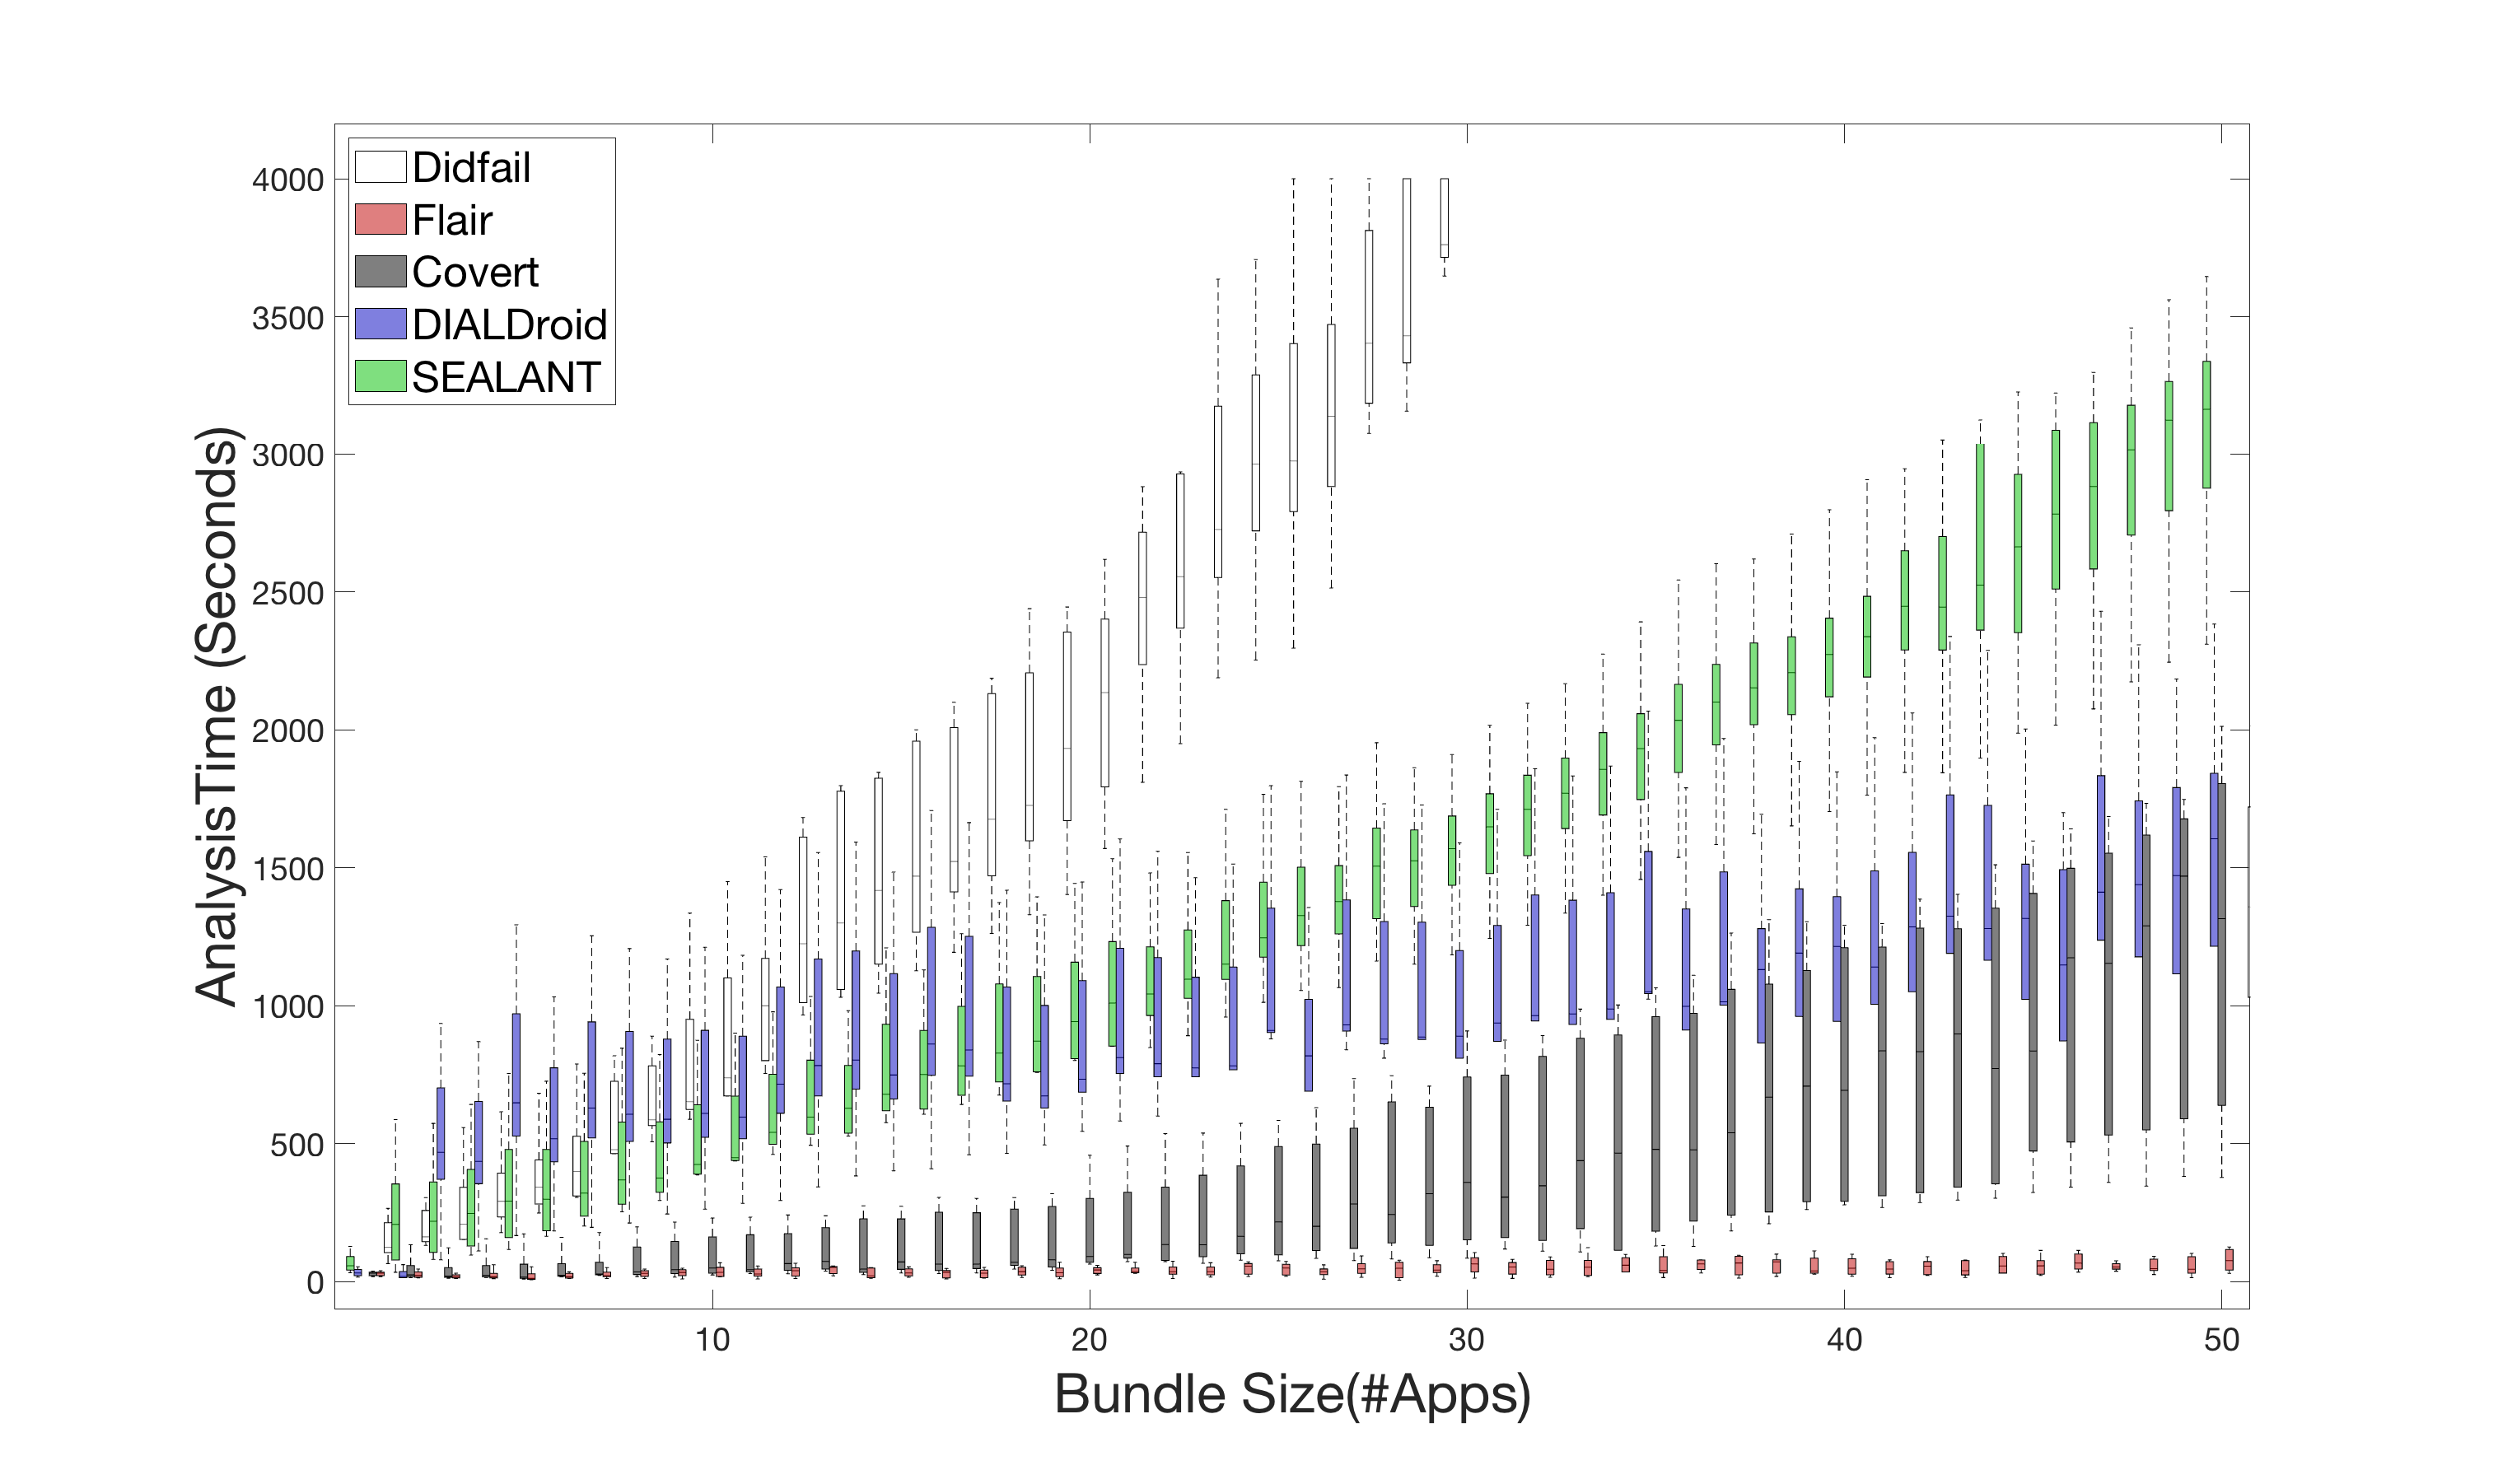
\includegraphics[width=\linewidth]{BoxPlotGraph}
	\label{figure:1}
	\caption{Box plot graphs showing tool analysis times for various tools.}
\end{figure*}


	%Average Analysis Time Graph
	\begin{figure}[H]
		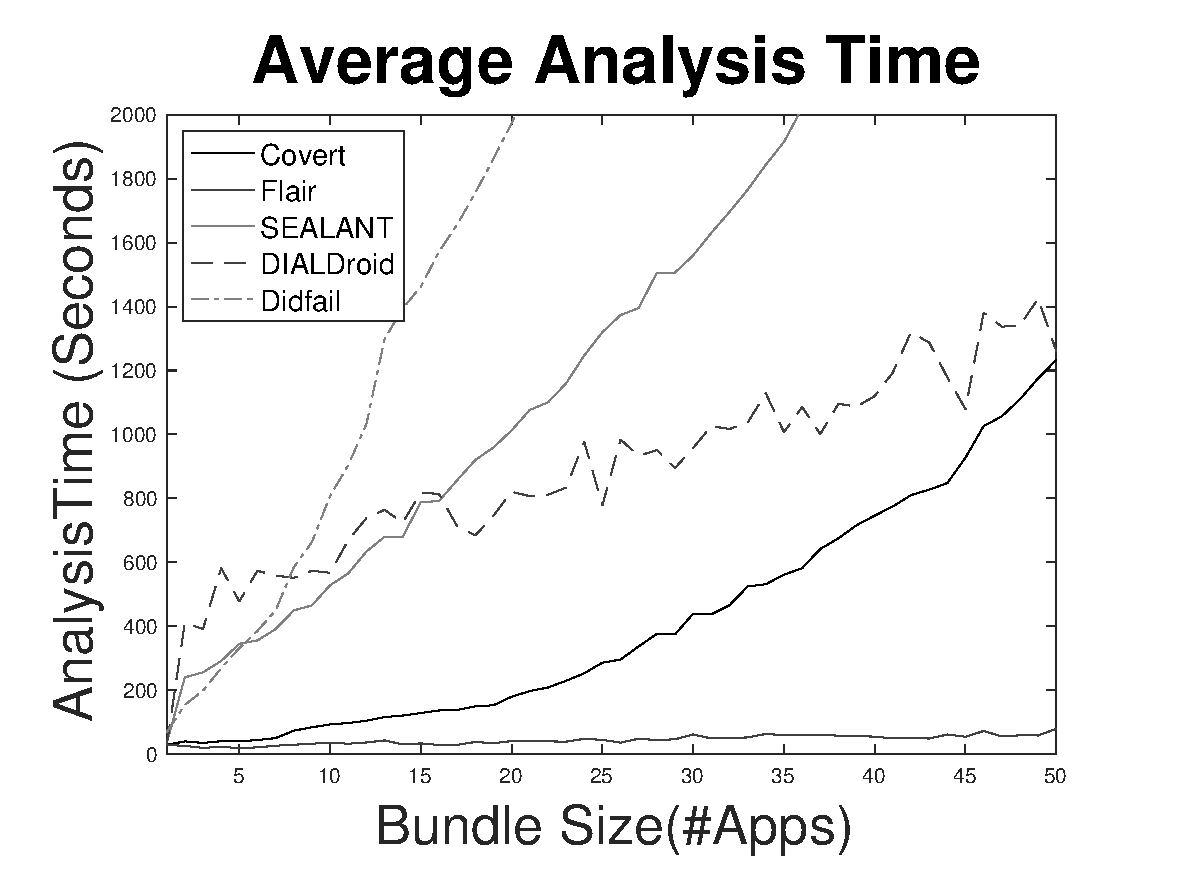
\includegraphics[width=\linewidth]{AverageGraph}
		\label{figure:2}
		\caption{Average analysis times for tools.}
	\end{figure}
	
	\subsection{RQ1:}
		We first look to evaluate the analysis time of Flair in relation to Covert, DIALDroid, and SEALANT. The box plot graphs presented in Figure 1 show the spread of analysis times for each tool. This data is presented in accordance with Figure 2 which represents the average analysis time of all tests run for all tools. These results show that Flair has a much smaller spread of analysis time across bundles, and much faster analysis times when analyzing bundles in an iterative fashion. Flair is able to analyze each application added to a bundle far faster since it only has to analyze the one application that was added, whereas the other tools analyze the entire bundle plus an additional application.\\
		It is shown in Figure 2 that SEALANT and Covert follow similar trends, except SEALANT shows much greater analysis times. This is most likely because SEALANT is built on top of Covert and runs Covert within its Analysis tool. In addition to Covert SEALANT also runs IC3 in its analyzer tool. The trend of covert is maintained in the data, but extra time is added with the addition of the IC3. DIALDroid follows a trend which appears to cause a great increase in time during the first few applications of a bundle. After those first few applications, DIALDroid increases at a much slower rate. Didfail's analysis times grows far faster than any of the other tools. Though it is not presented in \ref{figure:2}, Didfail fails to make it all the way to fifty applications. It could only get to thirty applications before failing to analyze any bundle that was larger. Flair maintains a near horizontal trend far below the other average times.\\
		
		To assess the rate of failure in the various tools we used the methods described in \ref{methods} to find the percentage of applications in each test which failed. The data we collected shows that while Covert, SEALANT, Didfail, and Flair do not fail to analyze any of the applications, DIALDroid failed a significant \textit{32.19 percent\textbf{(NOT FINAL NUMBER)}} of applications on average across all runs. This was primarily because DIALDroid would attempt to allocate more than our allotted 14 GB of memory, which was more than twice that allocated to any of the other tools. SEALANT, Covert, Didfail, and Flair all were able to run without any memory issues with far less memory. Therefore, Flair is able to analyze applications as reliably in terms of failure rate as well as SEALANT, Covert, and Didfail, while analyzing applications more reliably than DIALDroid.
		
	\subsection{RQ3:}
		text
	\subsection{Question 4:}
		text


\section[3]{Conclusion}
Here we will have a conclusion.


\end{document}

